\documentclass[journal]{IEEEtran}

% Correct bad hyphenation here
\hyphenation{op-tical net-works semi-conduc-tor}

\usepackage{float}
\usepackage{graphicx}
\usepackage{algorithm}
\usepackage{algorithmic}
\usepackage{amsmath}
\usepackage{color}
\usepackage{soul}
\usepackage{booktabs}
\usepackage{enumitem}
\usepackage{array} % For better table column control
\usepackage{url}
\usepackage{tikz}
\usetikzlibrary{positioning,arrows.meta}

\begin{document}
\small

% Paper title
\title{EcoTrust-DT: Digital-Twin Enabled Multi-Objective Carbon and Water-Aware Scheduling with Policy Enforcement for Privacy-Sensitive AI-Agent Workloads in Federated Cloud--Edge Systems: A WaterWise Pilot Reproduction and a Narrowed Research Gap}

\author{Muhammad Waseem Akhtar, Basharat Hussain\textsuperscript{*}, Syed Umar Javed
 \thanks{Muhammad Waseem Akhtar is pursuing his B.S. degree in Computer Science, FAST University (NUCES), Islamabad 44000, Pakistan (email: i221226@nu.edu.pk).}
 \thanks{Syed Umar Javed is pursuing his B.S. degree in Computer Science, FAST University (NUCES), Islamabad 44000, Pakistan (email: i210412@nu.edu.pk).}
 \thanks{Basharat Hussain is working with the Department of Computer Science, FAST University (NUCES), Islamabad 44000, Pakistan.}
 \thanks{\textsuperscript{*} Correspondence: basharat.hussain@isb.nu.edu.pk}
}

% The paper headers
\markboth{}%
{Muhammad Waseem Akhtar, Basharat Hussain, and Syed Umar Javed: EcoTrust-DT}

% make the title area
\maketitle

\begin{abstract}
The rapid growth of AI-agent and Large Language Model (LLM) workloads creates a dual challenge for cloud--edge infrastructure: large environmental footprints (carbon emissions and freshwater consumption) and strict enterprise privacy constraints. Traditional schedulers are mostly reactive, optimize single objectives such as cost or latency, and often overlook data-residency and confidential-computing requirements. This paper proposes \textbf{EcoTrust-DT}, a Digital-Twin-enabled, multi-objective scheduling framework for federated cloud--edge systems that applies hard policy filtering before predictive multi-objective placement and records every decision in a tamper-evident, hash-chained audit layer. Following a reproduction-first workflow, we also report a bounded pilot reproduction of WaterWise (PPoPP 2025), a carbon- and water-aware scheduler, using the official public code release in a CPU-only Linux environment. On the first 1,440 one-minute steps of the bundled Borg trace (16,707 arrivals) and with a deterministic numeric ordering of trace files, WaterWise produced 31.34\% lower modeled carbon output and 20.31\% lower modeled water output than the home-region baseline, while mean completion latency rose from 119.97~s to 127.81~s (+6.54\%) and the 95th-percentile latency stayed at 326.03~s in both arms. Code reading revealed several reproduction threats: unsorted trace enumeration with undocumented positional labels, a PuLP/CBC solver where the paper describes GLPK, a much smaller host than the artifact describes, and a single-day, single-seed scope. The result is therefore reported as a corrected-order diagnostic pilot, not a validated full reproduction. Building on it, we narrow EcoTrust-DT to a falsifiable question: whether a short-horizon digital-twin lookahead adds value over an otherwise identical current-telemetry carbon--water scheduler when hard residency, security, availability, and latency-SLO policies are enforced for bursty GPU inference. We specify the methodology, experimental arms, guardrail metrics, and limitations required before any improvement claim can be made. No EcoTrust-DT performance results are claimed in this paper.
\end{abstract}

\begin{IEEEkeywords}
Digital Twin, Green Cloud Computing, Carbon-Aware Scheduling, Water-Aware Scheduling, WaterWise, Reproducibility, AI-Agent Workloads, GPU Inference, Federated Cloud-Edge, Privacy-Preserving Computing, Policy-Constrained Scheduling, Multi-Objective Optimization, Trustworthy AI.
\end{IEEEkeywords}

\IEEEpeerreviewmaketitle

%==============================================================
\section{Introduction}
\IEEEPARstart{D}{ata-center} workload placement can materially change environmental impact because electricity carbon intensity, cooling water use, the water intensity of electricity generation, queue conditions, and site availability vary across regions and time. Carbon and water objectives can conflict: optimizing only one dimension may shift the burden rather than remove it. WaterWise addresses this trade-off by scheduling parallel jobs across geographically distributed data centers while accounting for carbon, water, delay tolerance, and regional water stress \cite{ref2}.

The rapid proliferation of Artificial Intelligence (AI) agents and LLM services has also transformed cloud--edge computing. This research lies at the intersection of several domains:
\begin{itemize}[leftmargin=*]
    \item Sustainable and green cloud computing
    \item Cloud--edge resource management
    \item AI infrastructure and GPU orchestration
    \item Digital Twin technology
    \item Privacy-preserving and policy-aware computing
    \item Multi-objective optimization
    \item Trustworthy AI and auditable cloud governance
\end{itemize}

EcoTrust-DT proposes a cloud--edge orchestration framework for AI-agent workloads such as LLM inference, document retrieval, tool calls, and batch processing. It uses a Digital Twin, a continuously updated virtual replica of cloud regions, edge nodes, GPUs, queues, networks, environmental conditions, and security capabilities, to predict the impact of scheduling decisions before execution. The framework first checks non-negotiable policies (data residency, privacy classification, confidential-computing requirements, water-stress restrictions, and latency service-level objectives). It then uses the Digital Twin to compare the allowed locations and choose the placement that best balances predicted carbon, freshwater consumption, cost, latency, queue delay, and operational risk.

The original EcoTrust-DT proposal states expected outcomes rather than completed empirical results. The required research workflow is therefore: reproduce a real baseline, document differences honestly, identify an evidence-backed gap, implement a focused improvement, and evaluate it against the reproduced baseline. This paper follows that workflow in a deliberately bounded manner. We select WaterWise as the base article because it is recent, appeared at a reputable ACM venue, addresses cloud scheduling, jointly considers carbon and water, and provides public code and artifact resources \cite{ref2,ref9,ref10}. We then perform a pilot reproduction and record reading notes from the code, configuration, input files, and output logs.

The contributions of this paper are fourfold. First, we document the execution environment, run configuration, and output logs for a one-day WaterWise pilot. Second, we report the reproduced carbon, water, latency, and scheduler-timing values and compare them with the published scope without overclaiming equivalence. Third, we record code-reading findings that affect reproducibility, including trace-ordering behavior, solver deviation, and undocumented input transformations. Fourth, we narrow EcoTrust-DT to a falsifiable research question about short-horizon forecast lookahead under hard policy constraints for latency-bounded GPU inference.

The remainder of the paper is organized as follows. Sections~II--VII give the team, problem, gap, research question, and objectives. Section~VIII reviews related work and Section~IX justifies the selected baseline. Section~X documents the reproduction environment and reading protocol, Section~XI describes the WaterWise method and input provenance, and Section~XII reports the pilot results and deviation analysis. Section~XIII identifies the candidate research gap, Section~XIV presents the EcoTrust-DT methodology, and Section~XV specifies the experimental design. Section~XVI discusses limitations and Section~XVII concludes.

%==============================================================
\section{Group and Roles}
This research is designed for a two-member team with clearly delineated, complementary responsibilities:
\begin{itemize}[leftmargin=*]
    \item \textbf{Member A --- Digital Twin and Cloud--Edge Simulation:} Develop the Digital Twin model, simulate multi-cloud and edge infrastructure, integrate environmental and infrastructure telemetry, create workload traces, and analyze prediction accuracy.
    \item \textbf{Member B --- Scheduling, Policy, and Trust:} Develop the policy engine, multi-objective scheduling algorithm, privacy and data-residency controls, tamper-evident audit log, and compliance/performance dashboard.
\end{itemize}

%==============================================================
\section{Approved Area and Title}
\begin{center}
\textbf{Area:} Digital-Twin Enabled Green, Trustworthy Cloud--Edge Computing for AI
\end{center}
\textbf{Title:} EcoTrust-DT: Digital-Twin Enabled Multi-Objective Carbon and Water-Aware Scheduling with Policy Enforcement for Privacy-Sensitive AI-Agent Workloads in Federated Cloud--Edge Systems

%==============================================================
\section{Problem and Motivation}
AI agents and LLM-powered services increasingly depend on GPU-based cloud infrastructure. Their operation consumes electricity, produces carbon emissions, and can require significant freshwater through data-center cooling and electricity generation. At the same time, enterprises handling confidential information cannot send prompts, documents, retrieved data, or tool-call inputs to any available cloud region because they must comply with privacy, data-residency, security, and audit requirements.

Traditional schedulers generally optimize a single target such as low cost, low latency, energy efficiency, or carbon reduction. This is insufficient because a low-carbon site may use more water, a low-cost site may be overloaded, and a fast site may violate privacy or regional-data rules. Conditions also change rapidly: GPU queues grow, carbon intensity varies, drought restrictions appear, prices change, and data centers or network links fail. A scheduler using only current telemetry may make a poor placement decision when conditions shift immediately afterward.

EcoTrust-DT addresses this challenge by using a Digital Twin to test feasible placement options virtually before execution. It can answer questions such as: \textit{Which policy-approved region is likely to meet the latency SLO with the lowest combined carbon and water impact?} Or: \textit{Should a workload be rerouted when a GPU shortage, carbon spike, drought restriction, or outage occurs?}

%==============================================================
\section{Initial Gap}
Existing research has important limitations that this proposal addresses:
\begin{enumerate}
    \item Many cloud schedulers optimize carbon emissions, cost, energy, or latency separately rather than jointly optimizing carbon and freshwater impact.
    \item Existing studies often focus on generic web services or batch jobs rather than AI-agent workflows involving LLM inference, retrieval, tool calls, sensitive documents, and heterogeneous GPU requirements.
    \item Policy enforcement, privacy, data residency, confidential-computing requirements, and auditable reasoning are often absent from sustainability-oriented scheduling systems.
    \item Multi-cloud and edge environments contain heterogeneous GPUs, variable networks, and rapidly changing resource conditions, creating complexity beyond traditional single-cloud scheduling.
    \item Current-telemetry schedulers react to the present system state but may not predict upcoming queue growth, carbon changes, water constraints, price changes, or failures.
    \item There is limited work on using a continuously synchronized Digital Twin to proactively evaluate these dynamic conditions while enforcing sustainability and governance constraints for privacy-sensitive AI-agent workloads.
\end{enumerate}
Section~XIII revisits this list after the baseline reproduction and narrows it to a candidate gap that can be tested.

%==============================================================
\section{Primary Research Question}
Can a continuously updated Digital Twin improve the carbon emissions, freshwater consumption, latency, cost, and policy-compliance performance of a policy-driven and verifiable scheduler for privacy-sensitive AI-agent workloads across federated cloud--edge systems, compared with schedulers that use only current telemetry?

This broad question is retained as the long-term direction. The testable, narrowed form used for the first experiments is stated in Section~XIII.

%==============================================================
\section{Objectives}
\begin{enumerate}
    \item Design a Digital Twin that represents multi-cloud regions, edge nodes, heterogeneous GPUs, network links, queues, workloads, environmental conditions, security capabilities, and site availability.
    \item Develop a multi-objective scheduling model that uses Digital-Twin predictions to jointly optimize carbon emissions, water consumption, latency, cost, queue delay, and privacy/operational risk.
    \item Implement policy enforcement and verifiable governance for data residency, workload classification, confidential-computing requirements, latency SLOs, drought thresholds, and tamper-evident audit records.
    \item Evaluate EcoTrust-DT against conventional, policy-aware, and sustainability-aware schedulers under normal workload conditions and stress situations such as GPU shortages, carbon spikes, drought periods, price surges, and regional outages.
\end{enumerate}

%==============================================================
\section{Related Work}

\subsection{Carbon- and Water-Aware Cloud Scheduling}
Sustainable cloud scheduling has evolved from energy-aware consolidation toward multi-resource environmental accounting. Early energy-aware allocation heuristics focused on data-center power management and virtual-machine placement \cite{ref8}. More recent systems recognize that carbon and water objectives can conflict. WaterWise explicitly co-optimizes carbon and water footprints for geographically distributed parallel workloads and shows that optimizing only one environmental dimension can harm the other \cite{ref2}. Moore et al.\ study sustainable carbon-aware and water-efficient LLM scheduling in geo-distributed cloud datacenters \cite{ref1}. CASPER examines carbon-aware scheduling and provisioning for distributed web services \cite{ref3}, while Sinan addresses ML-based and QoS-aware resource management for cloud microservices \cite{ref4}. These studies establish that sustainability-aware scheduling is an active area, but they do not jointly address hard privacy/residency policy, predictive digital-twin lookahead, and latency-bounded GPU inference in a single evaluated system.

\subsection{Digital Twins for Resource Orchestration}
Digital twins are virtual replicas that synchronize with physical systems to support monitoring, prediction, and what-if analysis \cite{ref5,ref6,ref7}. In edge computing, digital-twin-assisted task scheduling has been explored for end-to-end computing systems \cite{ref14}. However, a digital twin should not be claimed merely because a scheduler adds a weighted score. A credible digital-twin component requires an explicit state representation, forecast horizon, update cadence, prediction-error measurement, and feedback loop. EcoTrust-DT therefore adopts a minimum viable digital twin: a site-state snapshot plus a short-horizon predictor for queue delay and environmental intensity, evaluated against current-state scheduling and deliberately stale or noisy forecasts.

\subsection{Cloud--Edge Simulation and Reproducible Artifacts}
Reproducible simulation platforms are important for evaluating federated cloud--edge policies. EcoKube provides a heterogeneous edge-cloud simulator with policy comparisons and Kubernetes replay \cite{ref13}. CloudSim Plus supports multi-cloud, power- and network-aware simulation and trace-driven tasks \cite{ref12}. For the present study, WaterWise is preferred as the initial reproduction target because it has an author-associated public implementation and an archived software artifact \cite{ref9,ref10}. CloudSim Plus remains an alternative if a richer federation model is later required, but switching frameworks would make exact baseline replication less direct.

%==============================================================
\section{Selected Baseline and Reproducibility Rationale}
The selected base article is \textit{WaterWise: Co-optimizing Carbon- and Water-Footprint Toward Environmentally Sustainable Cloud Computing}, published in PPoPP 2025 \cite{ref2}. WaterWise satisfies the reproduction-first requirement: it has a public paper, official public code, an archived Zenodo artifact, documented run settings, workload traces, and sustainability metrics. Table~\ref{table:resources} summarizes the resources used.

WaterWise is not a perfect match for the full EcoTrust-DT vision. It does not model privacy-sensitive LLM inference, confidential-computing attestation, hash-chained audit, or a full federated cloud--edge digital twin. This mismatch is intentional and useful: WaterWise provides a reproducible sustainability baseline, while EcoTrust-DT is positioned as a focused extension that adds policy filtering and predictive lookahead.

\begin{table*}[!t]
\caption{Selected WaterWise Baseline Resources and Their Role in the Reproduction}
\label{table:resources}
\centering
\footnotesize
\renewcommand{\arraystretch}{1.15}
\begin{tabular}{|p{3.2cm}|p{5.2cm}|p{8.2cm}|}
\hline
\textbf{Resource} & \textbf{Role} & \textbf{Public locator} \\ \hline
WaterWise paper & Main article to reproduce & \url{https://doi.org/10.1145/3710848.3710891} \\ \hline
WaterWise arXiv version & Accessible manuscript for methodology inspection & \url{https://arxiv.org/abs/2501.17944} \\ \hline
Official public code & Implementation, scripts, optimizers, and run instructions & \url{https://github.com/LukeJYK/PPoPP25_WaterWise} \\ \hline
Zenodo artifact & Versioned software/data deposit used for reproduction & \url{https://zenodo.org/records/14583915} \\ \hline
Google Borg trace & Workload source cited by WaterWise & \url{https://github.com/google/cluster-data} \\ \hline
Alibaba cluster trace & Workload source cited by WaterWise & \url{https://github.com/alibaba/clusterdata} \\ \hline
\end{tabular}
\end{table*}

%==============================================================
\section{Reproduction Environment and Reading Protocol}
The baseline was run in a controlled environment, and the students maintained reading notes for each script, configuration flag, input file, and output field. This makes the reproduction trail auditable: the notes record what each module does, which fields are consumed, which assumptions are embedded in the code, and where deviations from the paper may arise. The system specification is summarized in Table~\ref{table:env}. The reproduction was performed in a CPU-only Linux environment because the baseline artifact emphasizes scheduler simulation and environmental accounting rather than GPU-accelerated training. The exact code version is recorded in the reproduction log.

The reproduction protocol follows three rules. First, the original WaterWise configuration is frozen before any extension is added. Second, at least one core published comparison is reproduced unchanged before the problem is modified. Third, any mismatch is treated as a result to be explained, not as a failure to be hidden.

\begin{table}[!t]
\caption{Reproduction Environment and Reading Protocol Specification}
\label{table:env}
\centering
\footnotesize
\renewcommand{\arraystretch}{1.1}
\begin{tabular}{|p{2.2cm}|p{5.7cm}|}
\hline
\textbf{Item} & \textbf{Specification} \\ \hline
Execution mode & CPU-only Linux x86-64 environment \\ \hline
CPU & Intel Xeon Platinum 8581C at 2.30 GHz \\ \hline
Visible CPUs & 1 logical CPU \\ \hline
Memory & 1.5 GiB RAM \\ \hline
GPU & None used \\ \hline
Python & 3.8.18 \\ \hline
Key libraries & NumPy 1.24.4, pandas 2.0.3, PuLP 2.9.0, Fire 0.7.0, tqdm 4.67.1 \\ \hline
Solver & PuLP PULP\_CBC\_CMD \\ \hline
License observed & Apache-2.0 \\ \hline
Trace window & First 1,440 one-minute steps of bundled Borg trace \\ \hline
Arrivals in window & 16,707 \\ \hline
Arms & Released base and waterwise optimizers \\ \hline
Settings & Delay threshold 0.5; seed 40; PUE 1.2; carbon/water weights 0.5/0.5; history weight 0.1; history window 10 \\ \hline
Run command & \texttt{python3 run\_waterwise\_pilot.py ./pilot-results} \\ \hline
Reading notes & Released README, optimizer scripts, trace reader, input profiles, and output JSON logs \\ \hline
Deviation log & Original expectation, observed value, absolute/relative difference, explanation \\ \hline
\end{tabular}
\end{table}

\subsection{Reading Notes from Code and Artifact Inspection}
The following notes were recorded before and during the pilot.
\begin{itemize}[leftmargin=*]
    \item The released README and run scripts were inspected to identify the two comparison arms: the home-region base optimizer and the released waterwise optimizer.
    \item The bundled Borg input contains ten files, \texttt{app1\_instances.csv} through \texttt{app10\_instances.csv}, each with 14,400 scalar rows. The values sum to 234,765 arrivals, of which the first 1,440 steps contain 16,707 arrivals.
    \item The default trace reader uses \texttt{os.listdir()} and attaches fixed workload labels by list position. In the observed runtime this returned app10 before app1. For the paired rerun, only the trace reader was overridden to sort numerically (app1--app10) before assigning the same fixed labels. The optimizer code and experiment parameters were unchanged.
    \item Carbon-intensity and electricity-water-intensity-factor inputs contain five regional series with 240 values per region. The code repeats each reading 60 times to align to minute steps.
    \item Wet-bulb inputs have unequal raw line counts: Zurich, Madrid, and Milan have 239 lines each; Oregon has 240; Mumbai has 79. The code repeats readings 60 times, except Mumbai where the effective repetition is 180. The source of the water-stress factors and the unequal raw series lengths are not explained in the artifact.
    \item Energy and execution-time profiles are provided for ten workloads. The code converts energy values by dividing by 3,600,000. The raw measurement units and transfer-latency units are not independently documented.
    \item The paper describes GLPK for its MILP solver, while the released Python optimizer calls PuLP's CBC command interface. This pilot therefore records a solver deviation rather than claiming exact solver parity.
    \item The Zenodo record is cited as the published artifact, but a separate Zenodo archive was not downloaded for this pilot; inputs came from the released code package.
\end{itemize}

%==============================================================
\section{WaterWise Method, Inputs, and Provenance}

\subsection{Core Accounting Model}
The baseline implementation focuses on WaterWise's essential contribution: selecting among geo-distributed sites while jointly considering carbon and water impact. For a job $j$ placed at site $i$, the project records energy, carbon, and water impacts as
\begin{align}
E_{i,j} &= P_{i,j} \times T_{i,j}, \\
\mathrm{CO_2e}_{i,j} &= E_{i,j} \times CI_i, \\
W^{\mathrm{direct}}_{i,j} &= E_{i,j} \times WUE_i, \\
W^{\mathrm{indirect}}_{i,j} &= E_{i,j} \times EWIF_i, \\
W^{\mathrm{total}}_{i,j} &= W^{\mathrm{direct}}_{i,j} + W^{\mathrm{indirect}}_{i,j}.
\end{align}
Here $E$ is energy, $P$ is power, $T$ is execution duration, $CI$ is carbon intensity, $WUE$ is water-usage effectiveness, and $EWIF$ is the electricity-water intensity factor. The official WaterWise code and artifact are treated as authoritative for exact units, normalizations, optimizer behavior, and scheduler semantics.

\subsection{Input Documentation}
WaterWise is a systems-scheduling study, so its inputs are workload traces and environmental time series rather than conventional train/validation/test image or text datasets. Table~\ref{table:inputs} documents the input categories and the provenance fields recorded after inspecting the artifact.

For the GPU-inference extension, Alibaba's public GPU trace is a more relevant workload source than general CPU traces because it describes a mix of training and inference workloads from a production cluster with over 6,500 GPUs \cite{ref11}. However, it does not by itself contain confidential prompts, legal residency labels, or true inference SLO classes. Those attributes must be introduced as synthetic annotations and clearly labeled as simulated assumptions. They must not be presented as observed properties of the trace.

\begin{table*}[!t]
\caption{Baseline Input Provenance and Documentation Requirements}
\label{table:inputs}
\centering
\footnotesize
\renewcommand{\arraystretch}{1.15}
\begin{tabular}{|p{2.5cm}|p{5.0cm}|p{9.1cm}|}
\hline
\textbf{Input} & \textbf{Observed structure} & \textbf{Source / processing and open issue} \\ \hline
Borg workload & \texttt{borg\_trace/app1\_instances.csv}--\texttt{app10\_instances.csv}; 14,400 scalar rows per file; 234,765 total arrivals & README names Google Borg; code reads with \texttt{header=None}. Exact trace version, filtering, and app-to-label mapping are not documented. No train/test split. \\ \hline
Carbon and EWIF data & \texttt{data/ci/} and \texttt{data/ewif/}; five regional series, 240 values per region & README names Electricity Maps as source; code repeats each reading 60 times to align to minute steps. Exact dates, units, missing-value handling, and source-data snapshots are not specified. \\ \hline
Wet bulb and water stress & \texttt{data/wet\_bulb/}; raw line counts: Zurich/Madrid/Milan 239 each, Oregon 240, Mumbai 79; \texttt{data/region\_mix\_2023.json} supplies WSF & README names Meteologix for wet-bulb data. Code repeats readings 60 times (Mumbai 180); the source of the WSF values and the unequal raw series lengths are not explained. \\ \hline
Energy, transfer, and sites & Ten workload energy/time profile pairs in \texttt{profile\_data/}; app-specific values in \texttt{data/transfer.json}; five regions, 35 nodes each & README says AWS m5.metal profiles. Code converts energy values by dividing by 3,600,000; raw measurement units and transfer-latency units are not independently documented. \\ \hline
\end{tabular}
\end{table*}

%==============================================================
\section{Reproduced Pilot Results and Deviation Analysis}
Table~\ref{table:pilot} reports raw aggregates from the generated JSON outputs. Both arms completed all 16,707 arrivals. Relative change is computed as (WaterWise $-$ base)/base; negative footprint changes indicate a lower modeled footprint. For latency, the completion-time field of each arm's output was used, and percentiles use the empirical output distribution. Footprint values are in the code's output units, with conversions inherited from the bundled profiles and not independently calibrated.

\begin{table}[!t]
\caption{One-Day Pilot: Home-Region Baseline versus WaterWise}
\label{table:pilot}
\centering
\footnotesize
\renewcommand{\arraystretch}{1.1}
\begin{tabular}{|p{2.5cm}|p{1.5cm}|p{1.6cm}|p{1.6cm}|}
\hline
\textbf{Metric} & \textbf{Base} & \textbf{WaterWise} & \textbf{Change} \\ \hline
Completed jobs & 16,707 & 16,707 & 0.00\% \\ \hline
Aggregate carbon output & 47,285.437 & 32,467.142 & $-31.34\%$ \\ \hline
Carbon per completed job & 2.83028 & 1.94333 & $-31.34\%$ \\ \hline
Aggregate water output & 1,140.100 & 908.581 & $-20.31\%$ \\ \hline
Water per completed job & 0.068241 & 0.054383 & $-20.31\%$ \\ \hline
Mean completion latency (s) & 119.967 & 127.814 & $+6.54\%$ \\ \hline
95th-percentile latency (s) & 326.028 & 326.028 & 0.00\% \\ \hline
WaterWise mean per-step timer (ms) & Not instrumented & 12.30 & Not comparable \\ \hline
\end{tabular}
\end{table}

For this single day and seed, under the deterministic numeric file ordering, WaterWise reduced simulator carbon and water totals but increased mean completion latency. Its internal per-step timer averaged 12.30~ms over 1,440 steps; the baseline does not emit a corresponding timer. Whole-process wall time is omitted because it was not captured for this corrected-order rerun. These figures are descriptive and do not support statistical or general workload claims.

The paper-to-pilot comparison is summarized in Table~\ref{table:paper}. The reported paper reductions (at least 21.91\% carbon and 14.78\% water across its evaluated delay-tolerance settings) are not directly comparable with this one-day pilot: the trace window, solver, machine, and trace ordering differ. The numerical gap is therefore intentionally marked not comparable, rather than subtracted. A full reproduction should use the official scripts and matched settings, preserve raw logs, and resolve the trace-label mapping before claiming replication.

Table~\ref{table:deviation} records the main deviations from the artifact description and their implications. A reproduction mismatch is not automatically a failure; it becomes a valid result when it is measured, reported, and investigated. Possible explanations include different hardware, library versions, dataset version, preprocessing, random seeds, missing script parameters, or incomplete documentation. The project therefore preserves stdout, output logs, dependency versions, and failed runs.

\begin{table*}[!t]
\caption{Published Findings versus the Corrected-Order Pilot}
\label{table:paper}
\centering
\footnotesize
\renewcommand{\arraystretch}{1.15}
\begin{tabular}{|p{3.0cm}|p{4.2cm}|p{4.6cm}|p{4.6cm}|}
\hline
\textbf{Measure} & \textbf{WaterWise paper / artifact} & \textbf{Pilot measured here} & \textbf{Difference / interpretation} \\ \hline
Carbon reduction vs.\ home-region baseline & At least 21.91\% across evaluated delay tolerances & 31.34\% for first-day slice, seed 40, threshold 0.5 & Not comparable: different scope, solver, host, and input ordering \\ \hline
Water reduction vs.\ home-region baseline & At least 14.78\% across evaluated delay tolerances & 20.31\% for first-day slice, seed 40, threshold 0.5 & Not comparable for the same reasons \\ \hline
Borg workload scope & Ten days; README reports over 230,000 jobs & 1,440 minutes; 16,707 arrivals completed in each arm & Pilot is a one-day subset, not the full evaluation \\ \hline
Latency and run time & No matched one-day latency/runtime value used here & Mean latency: 119.97~s (base), 127.81~s (WaterWise); p95: 326.03~s in both; WaterWise timer 12.30~ms/step & Descriptive pilot only; baseline has no matching internal timer \\ \hline
\end{tabular}
\end{table*}

\begin{table*}[!t]
\caption{Deviation Log for the WaterWise Pilot}
\label{table:deviation}
\centering
\footnotesize
\renewcommand{\arraystretch}{1.15}
\begin{tabular}{|p{2.2cm}|p{4.3cm}|p{4.3cm}|p{5.5cm}|}
\hline
\textbf{Deviation} & \textbf{Original/artifact expectation} & \textbf{Observed in pilot} & \textbf{Effect on claim} \\ \hline
Hardware & Five-core/16-GB artifact evaluation host & One visible logical CPU, 1.5 GiB RAM, no GPU & Limits run to a one-day subset; no full-scale timing claim \\ \hline
Python & Python 3.8.11 documented & Python 3.8.18 used & Minor version difference; possible numerical/library drift \\ \hline
Solver & Paper describes GLPK & PuLP/CBC used by released code & Solver deviation; optimization path may differ \\ \hline
Trace scope & Ten days, over 230,000 jobs & First 1,440 minutes, 16,707 jobs & Pilot is diagnostic, not full reproduction \\ \hline
Trace ordering & Undocumented app-to-label mapping & Default \texttt{os.listdir()} order corrected to numeric order & Result is a corrected-order diagnostic, not proof of authors' intended mapping \\ \hline
Artifact download & Zenodo artifact available & Released-code inputs used; Zenodo archive not separately downloaded & Input provenance is bound to the released code, not the artifact archive \\ \hline
Seeds/settings & Full evaluation sweep implied & One seed, one delay threshold & No statistical or general workload claim \\ \hline
\end{tabular}
\end{table*}

%==============================================================
\section{Evidence-Backed Gap and Narrowed Research Question}
The gap must be discovered after reading and reproducing the baseline, not invented merely because a digital twin sounds attractive. Based on the WaterWise paper, code, artifact, and reproduction notes, the following limitations are relevant to the EcoTrust-DT direction.
\begin{enumerate}
    \item \textbf{Workload scope.} WaterWise targets geographically distributed parallel jobs in cloud data centers. It does not primarily target privacy-sensitive AI-agent inference requests containing prompts, documents, retrieved data, or tool-call inputs.
    \item \textbf{Policy enforcement.} The baseline does not impose hard data-residency, confidentiality, attestation, or provider/region eligibility constraints before optimization.
    \item \textbf{Predictive state.} WaterWise uses environmental and workload information for scheduling, but it is not evaluated as a continuously synchronized digital twin that forecasts near-future queue delay, carbon intensity, water intensity, and availability over a short decision horizon.
    \item \textbf{Cloud--edge heterogeneity.} The broader EcoTrust-DT setting includes federated cloud--edge GPU resources, variable network latency, edge nodes, and site outages. These are not the central focus of the reproduced baseline.
    \item \textbf{Governance and audit.} Privacy-sensitive scheduling requires decision provenance. A hash-chained audit layer is not part of the reproduced WaterWise baseline.
\end{enumerate}

These observations should be framed as a scope extension rather than a criticism of WaterWise, which was not designed to solve privacy-sensitive AI-agent scheduling. The defensible gap is the specific integration and evaluation question: \textit{does forecast/lookahead scheduling add value over an otherwise identical policy-aware, carbon/water-aware scheduler for latency-bounded, bursty GPU inference, when forecast error and workload privacy labels are made explicit?}

This gap is a candidate to validate, not a literature-proven absence. Existing work already covers carbon-and-water-aware scheduling, digital-twin resource orchestration, and sustainability-aware heterogeneous edge-cloud policy evaluation. A focused related-work and artifact check with the supervisor is required before claiming novelty.

\textbf{Narrowed research question.} Under matched workload, site capacity, policy filter, and random seed, does a five-minute forecast of queue delay, carbon intensity, and water intensity reduce modeled carbon and water per completed GPU-inference request relative to current-state scheduling, while meeting a predeclared p95 latency SLO and placing no request at a policy-ineligible site?

The falsifiable expectation is that lookahead may help when conditions change predictably, but will provide little or no benefit when forecasts are uninformative. A result that lowers footprint while violating the latency SLO or a hard policy is a failure against this question. The policy labels and SLOs attached to public traces must be identified as synthetic unless independently sourced.

%==============================================================
\section{Proposed EcoTrust-DT Methodology}
The proposed contribution is deliberately narrower than the full vision. EcoTrust-DT is implemented as a policy-safe, one-step-ahead placement policy for latency-bounded GPU inference under forecast uncertainty. It preserves hard residency, security, and SLO eligibility as a non-negotiable filter and, among eligible sites, compares (1)~current-telemetry scheduling with (2)~a lightweight digital-twin lookahead that predicts queue delay and environmental intensity over a fixed short horizon. The framework is divided into interconnected components, shown in Fig.~\ref{fig:arch}.

\begin{figure}[!t]
\centering
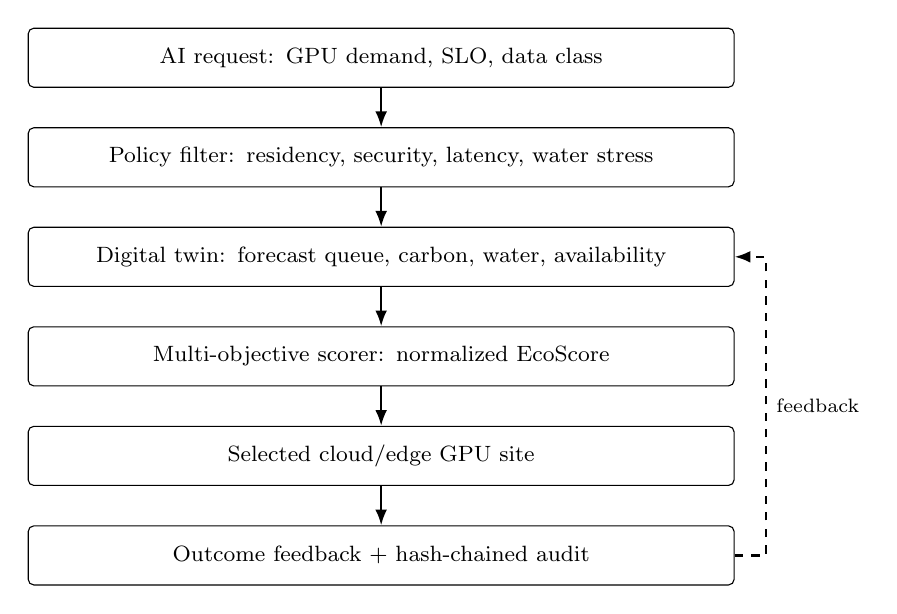
\begin{tikzpicture}[
  box/.style={draw, rounded corners=2pt, align=center, text width=0.72\columnwidth, minimum height=0.75cm, font=\footnotesize},
  arr/.style={-{Latex[length=2mm]}, thick},
  node distance=0.5cm]
\node[box] (a) {AI request: GPU demand, SLO, data class};
\node[box, below=of a] (b) {Policy filter: residency, security, latency, water stress};
\node[box, below=of b] (c) {Digital twin: forecast queue, carbon, water, availability};
\node[box, below=of c] (d) {Multi-objective scorer: normalized EcoScore};
\node[box, below=of d] (e) {Selected cloud/edge GPU site};
\node[box, below=of e] (f) {Outcome feedback + hash-chained audit};
\draw[arr] (a) -- (b);
\draw[arr] (b) -- (c);
\draw[arr] (c) -- (d);
\draw[arr] (d) -- (e);
\draw[arr] (e) -- (f);
\draw[arr, dashed] (f.east) -- ++(0.4,0) |- node[pos=0.25, right, font=\scriptsize]{feedback} (c.east);
\end{tikzpicture}
\caption{Narrowed EcoTrust-DT architecture. The diagram integrates baseline scheduling with policy filtering, predictive digital-twin feedback, and audit logging.}
\label{fig:arch}
\end{figure}

\subsection{AI-Agent Workload Model}
Each request is modeled as an AI-agent workflow with: arrival time; GPU-memory/GPU requirement; estimated service time (execution time); maximum acceptable latency or deadline (SLO); data class (public, internal, confidential, or restricted; synthetic in the evaluation); approved cloud providers and geographical regions; budget preference; carbon and water preference; and an optional confidential-computing or attestation requirement. Request contents are kept out of logs.

\subsection{Cloud--Edge Infrastructure Model}
A simulated federated environment is built using the WaterWise simulator for the reproduced baseline and CloudSim Plus or a comparable simulator if a richer federation model is required \cite{ref12}. It will include 3--6 cloud regions and several edge nodes with different GPU types, GPU memory, and available capacity; queue length and utilization; network latency to users; electricity/GPU cost; grid carbon intensity in gCO$_2$e/kWh; water-consumption factor in liters/kWh or liters/request; reliability and outage probability; and security capability, including confidential-computing support and attestation. The implementation distinguishes measured values, assumed values, and synthetic annotations.

\subsection{Environmental Telemetry and Site State}
The system collects or simulates dynamic information for each candidate site: carbon intensity, water-use intensity, electricity or GPU price, GPU availability, queue delay, network latency, drought or water-stress status, security and privacy capability, and availability or outage status.

\subsection{Hard Policy Filter}
The policy engine applies hard constraints before optimization, removing locations that are not allowed. Example policies: restricted data must run only in approved regions and providers; confidential workloads must run on attested or confidential-computing-capable resources; a workload must not be moved to a low-carbon site if predicted latency exceeds its SLO; high-water-use sites must be blocked if a drought or water-stress threshold is exceeded; and sensitive prompts or document contents must never be sent to an unapproved site. For request $r$ and site $i$, feasibility is
\begin{equation}
\begin{split}
F(i,r) = {} & \mathrm{Residency}(i,r) \wedge \mathrm{Security}(i,r) \wedge \mathrm{Latency}(i,r) \\
& \wedge \mathrm{WaterPolicy}(i,r) \wedge \mathrm{Available}(i),
\end{split}
\end{equation}
and the feasible site set is
\begin{equation}
S(r) = \{\, i \mid F(i,r) = 1 \,\}.
\end{equation}
Only sites in $S(r)$ may be scored, so a low environmental score can never override a privacy, legal, security, or data-residency requirement. The filter is tested as an invariant: a prohibited site can never win regardless of objective weights.

\subsection{Lightweight Digital Twin}
The Digital Twin is a virtual replica of the real or simulated cloud--edge system, continuously synchronized with infrastructure and environmental telemetry. The minimum viable twin is a state snapshot plus a short-horizon predictor. At time $t$, each site state is
\begin{equation}
\begin{split}
S_i(t) = [\,&\mathrm{GPU}_i, \mathrm{Queue}_i, \mathrm{Latency}_i, \mathrm{Carbon}_i, \\
&\mathrm{Water}_i, \mathrm{Price}_i, \mathrm{Availability}_i, \mathrm{Security}_i\,].
\end{split}
\end{equation}
The twin predicts the state at a near-future decision window $t+\Delta t$ and evaluates feasible placements (\textit{what-if} simulation) before committing a decision. After execution, actual outcomes are returned to the twin, which compares forecasts with real results and updates its estimation model. The initial predictor is intentionally transparent, such as a moving average or exponential smoother, rather than a deep learning model, which supports interpretability and makes forecast error easier to isolate. Prediction quality is measured by the mean absolute error
\begin{equation}
\mathrm{MAE} = \frac{1}{N}\sum_{k=1}^{N} \left| y_k - \hat{y}_k \right|.
\end{equation}
The project reports update cadence, prediction horizon, features, forecast errors, and what-if logic; a digital twin is not claimed merely by adding a weighted score.

\subsection{Multi-Objective Decision Score}
For every feasible site, the digital twin estimates predicted carbon, water, latency, cost, queue delay, and risk. The decision score is
\begin{equation}
\mathrm{EcoScore}(i,r) = \alpha \hat{C}_{i,r} + \beta \hat{W}_{i,r} + \gamma \hat{L}_{i,r} + \delta \hat{P}_{i,r} + \epsilon \hat{Q}_{i,r} + \zeta \hat{R}_{i,r},
\end{equation}
where all terms are normalized and
\begin{equation}
\alpha + \beta + \gamma + \delta + \epsilon + \zeta = 1.
\end{equation}
The selected site is
\begin{equation}
i^{*} = \arg\min_{i \in S(r)} \mathrm{EcoScore}(i,r).
\end{equation}
Weights reflect workload priorities: a confidential, real-time healthcare or banking request uses higher weights for latency and risk; a flexible batch AI task uses higher weights for carbon, water, and cost; a public request can prioritize affordability and performance while still observing sustainability targets. The project reports per-metric outcomes as well as the composite score and includes a sensitivity analysis over weights. A Pareto summary or constraint-based formulation is preferred when a single weighted score risks hiding trade-offs.

\begin{algorithm}[!t]
\caption{Policy-safe one-step-ahead placement}
\label{alg:placement}
\begin{algorithmic}[1]
\REQUIRE request $r$, current site state $S(t)$, forecast horizon $\Delta t$, weights $\theta$
\ENSURE placement decision and audit record
\STATE $S(r) \leftarrow \{i : F(i,r)=1\}$ \COMMENT{hard policy filter}
\IF{$S(r)=\emptyset$}
  \STATE queue or reject request; record reason
\ELSE
  \FOR{$i \in S(r)$}
    \STATE predict $\hat{q}_i, \hat{\ell}_i, \hat{c}_i, \hat{w}_i$ using digital twin
    \STATE compute normalized score $\mathrm{EcoScore}(i,r)$
  \ENDFOR
  \STATE $i^{*} \leftarrow \arg\min_{i \in S(r)} \mathrm{EcoScore}(i,r)$
  \STATE dispatch request to $i^{*}$
  \STATE observe actual outcome
  \STATE update twin and append hash-chained audit record
\ENDIF
\end{algorithmic}
\end{algorithm}

\subsection{Verifiable Audit Layer}
EcoTrust-DT creates a tamper-evident audit record for every decision. It is a small governance component, not a separate distributed-ledger contribution. Each record contains pseudonymous metadata: a privacy-preserving request identifier, workload data classification, policies checked, feasible sites after policy filtering, Digital-Twin predictions for candidate sites, selected site and decision reason, predicted and actual carbon/water/latency/cost values, SLO result, and rerouting or failure-recovery events. Records are hash-chained to detect later modification. The audit layer stores metadata and hashes rather than raw user prompts or sensitive retrieved documents.

%==============================================================
\section{Experimental Design and Evaluation Protocol}

\subsection{Paired Policy Arms}
The experiments keep workload arrivals, site capacities, carbon/water time series, policy labels, seeds, and all non-tested settings fixed across paired policy runs. This isolation is necessary because introducing many components simultaneously would make it difficult to determine which component caused any observed improvement. The minimum arms are listed in Table~\ref{table:arms}; they include FIFO/round-robin, carbon-only, water-only, policy-aware current-telemetry scheduling without a Digital Twin, and EcoTrust-DT. The conventional lowest-cost and lowest-latency schedulers are included as additional baselines in the full study.

\begin{table*}[!t]
\caption{Minimum Experimental Arms for Isolating the Contribution of Policy Filtering and Digital-Twin Lookahead}
\label{table:arms}
\centering
\footnotesize
\renewcommand{\arraystretch}{1.15}
\begin{tabular}{|p{1.0cm}|p{7.6cm}|p{7.8cm}|}
\hline
\textbf{Arm} & \textbf{Policy} & \textbf{Purpose} \\ \hline
A0 & WaterWise original configuration & Reproduced reference; retained unchanged \\ \hline
A1 & FIFO / round robin & Simple non-sustainability sanity baseline \\ \hline
A2 & Current-state carbon + water + latency score with hard policy filtering & Main fair comparator without lookahead \\ \hline
A3 & A2 plus forecast/lookahead digital twin & Proposed treatment; isolates predictive contribution \\ \hline
A4 & A3 with prediction disabled, stale, or error-injected & Ablation and forecast-value test \\ \hline
A5 & Carbon-only and water-only variants & Shows objective trade-off \\ \hline
\end{tabular}
\end{table*}

\subsection{Workloads and Scenarios}
\textbf{Workload conditions:} low, medium, and high request rates; public, internal, confidential, and restricted requests; short real-time inference and longer batch jobs; different latency SLOs and GPU requirements. \textbf{Stress conditions:} bursty arrivals, carbon-intensity spikes or shifts, drought or water-stress restrictions, GPU shortages, queue congestion, electricity-price surges, network degradation, forecast staleness/error, regional cloud or edge-node outages, and sudden AI-agent workload bursts. The narrowed study prioritizes bursts, forecast/queue errors, water/carbon changes, policy exclusions, and one outage case. Synthetic policy classes are explicitly labeled as simulated assumptions.

\subsection{Metrics and Hypothesized Outcomes}
The evaluation measures success across several dimensions. The metrics and the hypothesized (not yet observed) outcomes are given in Table~\ref{table:metrics}, and the reporting rules for primary and guardrail metrics are given in Table~\ref{table:primary}.

\begin{table}[H]
\caption{Evaluation Dimensions and Hypothesized Outcomes}
\label{table:metrics}
\centering
\renewcommand{\arraystretch}{1.1}
\resizebox{\columnwidth}{!}{%
\begin{tabular}{|p{2.0cm}|p{3.5cm}|p{5.5cm}|}
\hline
\textbf{Dimension} & \textbf{Metric} & \textbf{Hypothesized Outcome} \\ \hline
Sustainability & CO$_2$e per 1,000 requests & Lower carbon impact than FIFO, cost-only, and latency-only baselines \\ \hline
Sustainability & Liters of water per 1,000 requests & Lower freshwater impact without merely shifting harm from carbon to water \\ \hline
Performance & p95 end-to-end latency & Remains within defined SLO targets for real-time workloads \\ \hline
Reliability & SLO-miss rate & Low miss rate, including during stress conditions \\ \hline
Business & Cost per 1,000 requests & Competitive cost compared with performance-only scheduling \\ \hline
Trust & Policy-violation rate & Zero by construction, since policies filter sites before optimization \\ \hline
Auditability & Percentage of complete, verifiable audit records & High audit coverage for every placement decision \\ \hline
Resilience & Recovery time after outage & Faster rerouting and recovery than non-predictive baselines \\ \hline
Digital Twin & Carbon prediction error & Decreases as the Digital Twin receives execution feedback \\ \hline
Digital Twin & Water prediction error & Decreases as water and workload estimates are refined \\ \hline
Digital Twin & Latency prediction error & Lower error than simple current-state estimates \\ \hline
Digital Twin & Best-site selection accuracy & Higher rate of selecting the best feasible site \\ \hline
Digital Twin & Adaptation time & Quick reaction to outages, queues, carbon spikes, price changes, and drought restrictions \\ \hline
Digital Twin & Scheduling overhead & Low enough to remain practical for real-time decisions \\ \hline
\end{tabular}%
}
\end{table}

\begin{table*}[!t]
\caption{Primary and Guardrail Metrics for the EcoTrust-DT Evaluation}
\label{table:primary}
\centering
\footnotesize
\renewcommand{\arraystretch}{1.15}
\begin{tabular}{|p{2.4cm}|p{6.2cm}|p{8.0cm}|}
\hline
\textbf{Metric group} & \textbf{Metric} & \textbf{Reporting rule} \\ \hline
Sustainability & Carbon per completed request; water per completed request & Report run-level means and uncertainty across independent seeds \\ \hline
Performance & p50/p95/p99 end-to-end latency; SLO attainment/violations & Tail latency is a guardrail, not a tradeable weighted objective \\ \hline
Reliability & Throughput; rejected/queued requests; recovery time after outage & Report under normal and stress scenarios \\ \hline
Policy & Policy-violation count & Must be zero by construction, with automated tests \\ \hline
Efficiency & Scheduler decision overhead; GPU utilization & Report decision time and resource use \\ \hline
Twin quality & Predictor MAE for queue delay and carbon/water input & Report forecast error and staleness effects \\ \hline
Accounting & Energy/water-accounting assumptions & Disclose model factors and missing region-level observability \\ \hline
\end{tabular}
\end{table*}

\subsection{Interpretation Rules}
The study pre-registers the direction of the hypothesis, not the result. The expected direction is that forecastable, changing conditions may reduce carbon and water per completed request relative to current-state scheduling, while little or no benefit is expected when forecasts are uninformative. Latency-SLO failures and policy violations are guardrails. The following rules are used.
\begin{itemize}[leftmargin=*]
    \item If the lookahead arm improves environmental metrics but breaks p95 latency or policy invariants, it fails the stated goal.
    \item If the lookahead and current-state policy arms are statistically indistinguishable, the tested predictor adds no demonstrated value in the tested regime.
    \item If gains occur only with oracle-quality forecasts, the required forecast accuracy is quantified.
    \item Carbon and water numbers are reported as estimates tied to the disclosed energy model and water-intensity source, not as direct physical measurements unless measured instrumentation is used.
\end{itemize}

%==============================================================
\section{Limitations and Next Steps}
Several limitations must be stated explicitly.
\begin{enumerate}
    \item \textbf{Pilot versus full reproduction.} The reported run is a one-day, one-seed, corrected-order diagnostic pilot. It does not reproduce the full WaterWise evaluation and should not be presented as exact replication.
    \item \textbf{Hardware and solver differences.} The host has one visible logical CPU and 1.5~GiB RAM, and the optimizer used PuLP/CBC rather than the GLPK solver described in the paper. These differences affect runtime and may affect optimization paths.
    \item \textbf{Undocumented input mapping.} The default trace reader uses unsorted directory enumeration and positional workload labels. The numeric-order correction makes the pilot internally consistent, but the artifact does not document the intended app-to-label mapping.
    \item \textbf{Modeled environmental values.} Energy-to-carbon and energy-to-water calculations are modeled estimates tied to disclosed factors and intensity sources, not direct physical measurements unless instrumented testbeds are used.
    \item \textbf{Synthetic privacy labels.} Neither the Alibaba nor the Google cluster traces contain confidential prompts/documents, legal residency labels, or true SLO classes needed to establish privacy compliance. These attributes are synthetic annotations and must not be presented as observed trace properties.
    \item \textbf{Simulation scope.} EcoTrust-DT is initially a simulation-based research prototype. Confidential computing is modeled as a site-eligibility capability unless actual attestation hardware is tested.
    \item \textbf{Novelty risk.} The gap is a candidate gap, not a proven absence. Close prior art includes WaterWise, EcoKube, digital-twin edge scheduling, and carbon/water-aware LLM scheduling. The final novelty claim must be refined with the supervisor after a focused related-work and artifact check.
\end{enumerate}
Before presenting EcoTrust-DT as a contribution, the team should: (1)~reproduce at least one complete official WaterWise result with the intended trace and threshold sweep; (2)~record artifact version, dataset provenance, checksums, exact commands, and all environment differences; (3)~validate the candidate gap against current related work, including sustainable LLM scheduling; (4)~implement the policy filter and forecast module as separately ablatable components; and (5)~run matched repeated experiments with disclosed synthetic assumptions. Any remaining difference from WaterWise's reported values should be explained, not tuned away.

%==============================================================
\section{Conclusion}
This paper proposed EcoTrust-DT, a framework that moves cloud--edge scheduling from a reactive, single-objective paradigm toward a proactive, multi-objective, policy-enforced design, and presented a bounded reproduction of WaterWise used to narrow the research direction. The pilot showed that, on the first 1,440 minutes of the bundled Borg trace and under a deterministic numeric trace ordering, WaterWise reduced modeled carbon output by 31.34\% and modeled water output by 20.31\% relative to the home-region baseline, while increasing mean completion latency by 6.54\% and leaving p95 latency unchanged. Because the run used a constrained host, one seed, one delay threshold, a corrected trace order, and PuLP/CBC rather than the paper-described GLPK solver, these values are reported as a diagnostic pilot rather than a full reproduction.

The reading notes identified concrete reproducibility issues: an undocumented app-to-label mapping, unsorted directory enumeration in the default loader, incomplete provenance for environmental series, and solver deviation. These issues prevent overclaiming and define the baseline that any EcoTrust-DT extension must respect.

The EcoTrust-DT contribution was therefore narrowed to a testable question: whether a short-horizon digital-twin lookahead improves carbon and water outcomes over an otherwise identical current-telemetry, policy-aware scheduler for latency-bounded GPU inference, without violating hard residency, security, availability, or SLO constraints. The final research claim must be earned through controlled experiments, ablations, and honest deviation reporting. If the lookahead module improves environmental metrics while preserving latency and policy guardrails, the contribution is a validated extension. If it does not, the negative result is still valuable because it identifies the forecast accuracy and workload regimes required for digital-twin scheduling to matter.

\section*{Acknowledgment}
The authors thank the research supervisor for guidance on reproduction scope, gap validation, and experimental design.

% References section - STRICTLY PLACED AT THE VERY END
\begin{thebibliography}{99}

\bibitem{ref1} H. Moore, S. Qi, N. Hogade, D. Milojicic, C. Bash, and S. Pasricha, ``Sustainable Carbon-Aware and Water-Efficient LLM Scheduling in Geo-Distributed Cloud Datacenters,'' in \textit{Proc. Great Lakes Symp. VLSI (GLSVLSI '25)}, 2025, pp. 929--934, doi: 10.1145/3716368.3735301.

\bibitem{ref2} Y. Jiang, R. Basu Roy, R. Kanakagiri, and D. Tiwari, ``WaterWise: Co-optimizing Carbon- and Water-Footprint Toward Environmentally Sustainable Cloud Computing,'' in \textit{Proc. 30th ACM SIGPLAN Annual Symp. Principles and Practice of Parallel Programming (PPoPP '25)}, 2025, pp. 297--311, doi: 10.1145/3710848.3710891.

\bibitem{ref3} A. Souza, S. Jasoria, B. Chakrabarty, A. Bridgwater, A. Lundberg, F. Skogh, A. Ali-Eldin, D. Irwin, and P. Shenoy, ``CASPER: Carbon-Aware Scheduling and Provisioning for Distributed Web Services,'' in \textit{Proc. 14th Int. Green and Sustainable Computing Conf. (IGSC '23)}, Toronto, ON, Canada, 2023, doi: 10.1145/3634769.3634812.

\bibitem{ref4} Y. Zhang, W. Hua, Z. Zhou, G. E. Suh, and C. Delimitrou, ``Sinan: ML-Based and QoS-Aware Resource Management for Cloud Microservices,'' in \textit{Proc. 26th ACM Int. Conf. Architectural Support for Programming Languages and Operating Systems (ASPLOS '21)}, 2021, pp. 167--181, doi: 10.1145/3445814.3446693.

\bibitem{ref5} F. Tao, H. Zhang, A. Liu, and A. Y. C. Nee, ``Digital Twin in Industry: State-of-the-Art,'' \textit{IEEE Trans. Ind. Informat.}, vol. 15, no. 4, pp. 2405--2415, 2019, doi: 10.1109/TII.2018.2873186.

\bibitem{ref6} A. Fuller, Z. Fan, C. Day, and C. Barlow, ``Digital Twin: Enabling Technologies, Challenges and Open Research,'' \textit{IEEE Access}, vol. 8, pp. 108952--108971, 2020, doi: 10.1109/ACCESS.2020.2998358.

\bibitem{ref7} W. Kritzinger, M. Karner, G. Traar, J. Henjes, and W. Sihn, ``Digital Twin in Manufacturing: A Categorical Literature Review and Classification,'' \textit{IFAC-PapersOnLine}, vol. 51, no. 11, pp. 1016--1022, 2018, doi: 10.1016/j.ifacol.2018.06.244.

\bibitem{ref8} A. Beloglazov, J. Abawajy, and R. Buyya, ``Energy-Aware Resource Allocation Heuristics for Efficient Management of Data Centers for Cloud Computing,'' \textit{Future Generation Computer Systems}, vol. 28, no. 5, pp. 755--768, 2012, doi: 10.1016/j.future.2011.08.004.

\bibitem{ref9} Y. Jiang, R. Basu Roy, R. Kanakagiri, and D. Tiwari, ``PPoPP25\_WaterWise,'' GitHub repository, 2025. [Online]. Available: \url{https://github.com/LukeJYK/PPoPP25_WaterWise}

\bibitem{ref10} Y. Jiang, R. Basu Roy, R. Kanakagiri, and D. Tiwari, ``WaterWise: Co-optimizing Carbon- and Water-Footprint Toward Environmentally Sustainable Cloud Computing (Version 3),'' Zenodo, 2025, doi: 10.5281/zenodo.14583915.

\bibitem{ref11} Alibaba Cluster Data, ``Cluster trace GPU v2020: README,'' 2020. [Online]. Available: \url{https://github.com/alibaba/clusterdata/blob/master/cluster-trace-gpu-v2020/README.md}. Accessed: Oct. 11, 2026.

\bibitem{ref12} CloudSim Plus Project, ``CloudSim Plus: A Java Object-Oriented Simulation Framework for Cloud and Fog Computing,'' GitHub, 2026. [Online]. Available: \url{https://github.com/cloudsimplus/cloudsimplus}

\bibitem{ref13} Large-scale Sustainable Computing Lab, ``EcoKube: Heterogeneous Edge-Cloud Simulation and Kubernetes Replay,'' GitHub, 2026. [Online]. Available: \url{https://github.com/g-uva/EcoKube}

\bibitem{ref14} R.-R. Zhong, Y.-X. Feng, X.-J. Song \textit{et al.}, ``Edge Computing Empowered Digital Twin: An End-to-End Computing Task Scheduling Approach,'' in \textit{Proc. 2024 IEEE 20th Int. Conf. Automation Science and Engineering (CASE)}, 2024, doi: 10.1109/CASE59546.2024.10711331.

\end{thebibliography}

\end{document}